% =============================================================================
% CE2031 Digital IC Design - Project 23
% Traffic Light Controller FSM with Emergency Override
%
%     Nhom5_LETHANHDANH_FINAL.tex  this file
%     results.tex                  measured numbers (written by make_figures.py)
%     figures/wave_emg.tex         TikZ timing diagrams drawn from the VCD file
%     figures/wave_ped.tex
%     figures/gtkwave_T*.png       GTKWave captures (capture_gtkwave.ps1)
%     photos/board_B1.jpg ... board_B9.jpg   board photographs (cropped;
%                                            originals in photos/raw/)
%
% Rebuild everything (from project23_traffic\):
%     .\run_sim.ps1
%     .\run_modelsim.ps1
%     cd quartus; F:\merged_partition_content\altera\quartus\bin64\quartus_sh -t run_quartus.tcl; cd ..
%     python paper\make_figures.py
%     .\paper\capture_gtkwave.ps1
%     cd paper; pdflatex Nhom5_LETHANHDANH_FINAL.tex   (twice)
%
% Draft marks: items that still need the authors (board photographs and
% observations, group number) are tagged [V1]..[V3] in red and listed on a
% checklist page at the end. \draftmarksfalse removes the tags and the page.
% =============================================================================
\documentclass[conference]{IEEEtran}
\usepackage[T1]{fontenc}
\renewcommand{\ttdefault}{lmtt}          % scalable typewriter font for the code
\usepackage{cite}
\usepackage{amsmath,amssymb}
\usepackage{graphicx}
\usepackage{xcolor}
\usepackage{booktabs}
\usepackage{array}
\usepackage{multirow}
\usepackage{listings}
\usepackage{url}
\usepackage{textcomp}
\usepackage{pifont}                       % circled numbers of the waveform
\usepackage{tikz}
\usetikzlibrary{arrows.meta,positioning,shapes.geometric,calc,fit}
\usepackage[hidelinks]{hyperref}

\graphicspath{{figures/}}

\newif\ifdraftmarks
\draftmarkstrue                          % \draftmarksfalse = version to hand in

\newcommand{\verify}[1]{\ifdraftmarks\,\textcolor{red}{\textbf{[#1]}}\fi}
\newcommand{\code}[1]{\texttt{\upshape #1}}
\newcommand{\st}[1]{\textsf{#1}}         % state name

% Generated by make_figures.py - do not edit.
% Sources: logs/*.log, logs/enc_*/*, logs/timing/*.rpt, quartus/output_files/*.rpt
\newcommand{\SimSeeds}{1, 7, 2026}
\newcommand{\SimCycles}{34{,}254}
\newcommand{\SimCyclesAll}{102{,}762}
\newcommand{\DirChecks}{305}
\newcommand{\DirCycles}{4{,}253}
\newcommand{\RandomCycles}{30{,}000}
\newcommand{\GoldenCycles}{102{,}762}
\newcommand{\HitSafe}{102{,}478}
\newcommand{\HitEmg}{250}
\newcommand{\HitYel}{1{,}961}
\newcommand{\HitOnehot}{102{,}478}
\newcommand{\HitPed}{7{,}888}
\newcommand{\HitAllred}{208}
\newcommand{\HitGmax}{1{,}961}
\newcommand{\HitYlen}{1{,}934}
\newcommand{\ArcA}{102}
\newcommand{\ArcB}{1{,}601}
\newcommand{\ArcC}{909}
\newcommand{\ArcD}{108}
\newcommand{\ArcE}{891}
\newcommand{\ArcF}{10}
\newcommand{\ArcG}{225}
\newcommand{\ArcH}{656}
\newcommand{\ArcI}{73}
\newcommand{\ArcJ}{1{,}427}
\newcommand{\ArcK}{877}
\newcommand{\ArcL}{80}
\newcommand{\ArcM}{866}
\newcommand{\ArcN}{12}
\newcommand{\ArcO}{247}
\newcommand{\ArcP}{607}
\newcommand{\ArcQ}{15}
\newcommand{\ArcR}{243}
\newcommand{\ArcS}{268}
\newcommand{\ArcT}{229}
\newcommand{\ArcU}{5}
\newcommand{\ArcV}{60}
\newcommand{\ArcW}{96}
\newcommand{\ArcX}{68}
\newcommand{\ArcMin}{5}
\newcommand{\ArcMinName}{\st{RECOVER}$\to$\st{EMG}}
\newcommand{\StA}{943}
\newcommand{\StB}{1{,}011}
\newcommand{\StC}{891}
\newcommand{\StD}{995}
\newcommand{\StE}{950}
\newcommand{\StF}{866}
\newcommand{\StG}{532}
\newcommand{\StH}{230}
\newcommand{\StI}{229}
\newcommand{\MutErrA}{39}
\newcommand{\MutViolA}{41}
\newcommand{\MutPropsA}{\code{a\_yel}}
\newcommand{\MutGoldA}{6{,}738}
\newcommand{\MutErrB}{9}
\newcommand{\MutViolB}{0}
\newcommand{\MutPropsB}{--}
\newcommand{\MutGoldB}{21{,}096}
\newcommand{\MutErrC}{33}
\newcommand{\MutViolC}{0}
\newcommand{\MutPropsC}{--}
\newcommand{\MutGoldC}{23{,}318}
\newcommand{\MutErrD}{125}
\newcommand{\MutViolD}{0}
\newcommand{\MutPropsD}{--}
\newcommand{\MutGoldD}{24{,}762}
\newcommand{\MutErrE}{0}
\newcommand{\MutViolE}{11{,}012}
\newcommand{\MutPropsE}{\code{a\_safe}, \code{a\_yel}}
\newcommand{\MutGoldE}{10{,}649}
\newcommand{\MutErrF}{17}
\newcommand{\MutViolF}{36}
\newcommand{\MutPropsF}{\code{a\_ylen}}
\newcommand{\MutGoldF}{6{,}128}
\newcommand{\MsimVersion}{10.1d}
\newcommand{\LEBin}{254}
\newcommand{\FFBin}{100}
\newcommand{\FmaxBin}{112.46}
\newcommand{\BitsBin}{4}
\newcommand{\LEGray}{247}
\newcommand{\FFGray}{100}
\newcommand{\FmaxGray}{118.02}
\newcommand{\BitsGray}{4}
\newcommand{\LEHot}{230}
\newcommand{\FFHot}{101}
\newcommand{\FmaxHot}{130.98}
\newcommand{\BitsHot}{9}
\newcommand{\LEFsm}{48}
\newcommand{\FFFsm}{18}
\newcommand{\LEDiv}{44}
\newcommand{\FFDiv}{28}
\newcommand{\LEStrobe}{31}
\newcommand{\FFStrobe}{18}
\newcommand{\LETimer}{26}
\newcommand{\FFTimer}{8}
\newcommand{\LEBcd}{24}
\newcommand{\FFBcd}{0}
\newcommand{\LEDb}{5}
\newcommand{\FFDb}{5}
\newcommand{\LEtopOwn}{32}
\newcommand{\FFtopOwn}{3}
\newcommand{\LEtotal}{230}
\newcommand{\NumRegisters}{101}
\newcommand{\NumPins}{106}
\newcommand{\MemBits}{0}
\newcommand{\ClockGlobal}{GCLK2}
\newcommand{\QuartusVersion}{13.0.1}
\newcommand{\EncFinal}{One-Hot}
\newcommand{\FmaxSlow}{130.98}
\newcommand{\FmaxFast}{288.6}
\newcommand{\SlackSetup}{12.365}
\newcommand{\SlackTen}{2.365}
\newcommand{\CritDelay}{7.671}
\newcommand{\CritFrom}{cnt[3] (state\_timer)}
\newcommand{\CritTo}{cnt[1] (state\_timer)}
\newcommand{\SlackHold}{0.391}
\newcommand{\SlackRecovery}{17.674}
\newcommand{\SlackRemoval}{1.232}
%% T5 event times (GTKWave markers A..E), in clock cycles
\newcommand{\WaveDbLat}{5}
\newcommand{\WaveYellow}{12}
\newcommand{\WaveRecover}{8}


% ---- SystemVerilog listings ---------------------------------------------------
\lstdefinelanguage{SystemVerilog}[]{Verilog}{
  morekeywords={logic,always_comb,always_ff,unique,priority,int,bit,localparam,
                timeunit,timeprecision,automatic,assert,property,endtask,endfunction},
}
\lstset{
  language=SystemVerilog,
  basicstyle=\ttfamily\scriptsize,
  keywordstyle=\bfseries,
  commentstyle=\itshape,
  numbers=left, numberstyle=\tiny, numbersep=4pt,
  xleftmargin=1.4em, frame=lines, framesep=2pt,
  columns=fixed, basewidth=0.48em,
  keepspaces=true, showstringspaces=false,
  upquote=true,
  captionpos=b,
}

% ---- TikZ styles ----------------------------------------------------------------
\tikzset{
  >=Stealth,
  blk/.style={draw, thick, minimum height=8mm, minimum width=17mm, align=center, font=\footnotesize},
  sm/.style={draw, thick, circle, minimum size=11mm, inner sep=0pt, align=center, font=\scriptsize},
  lbl/.style={font=\tiny, fill=white, inner sep=1pt},
  sig/.style={font=\scriptsize},
}

% ---- Board photograph ----------------------------------------------------------
\newcommand{\boardphoto}[2]{%
  \IfFileExists{photos/board_B#1.jpg}{%
    \includegraphics[width=\linewidth]{photos/board_B#1.jpg}%
  }{\IfFileExists{photos/board_B#1.png}{%
    \includegraphics[width=\linewidth]{photos/board_B#1.png}%
  }{%
    \typeout{*** MISSING PHOTO B#1: photos/board_B#1.jpg (or .png)}%
    \begingroup\setlength{\fboxsep}{0pt}%
    \textcolor{red}{\fbox{\parbox[c][0.62\linewidth][c]{\dimexpr\linewidth-2\fboxrule\relax}{%
      \centering\scriptsize\color{black}%
      \textcolor{red}{\textbf{MISSING PHOTO B#1}}\\[3pt]
      #2\\[3pt]
      \code{photos/board\_B#1.jpg}}}}%
    \endgroup
  }}%
}

\begin{document}

\title{Design and Verification of a Traffic Light Controller FSM with Emergency
       Override on a Cyclone~II FPGA}

\author{\IEEEauthorblockN{Le Thanh Danh and Phan Duy Luan}
\IEEEauthorblockA{Group 5\verify{V1}, CE2031 Digital IC Design, Project 23\\
Vietnam--Korea University of Information and Communication Technology (VKU)\\
The University of Danang, Da Nang, Vietnam}}

\maketitle

\begin{abstract}
This report presents a traffic light controller for a two-road intersection,
written in SystemVerilog as a 9-state Moore finite-state machine, with pedestrian
service, green extension when the other road is empty, and an emergency override:
an emergency request ends a green through a full yellow and then holds every
direction at red until the request is released. The time base is restarted at
every phase change, so every phase, including a yellow forced by an emergency,
lasts exactly its programmed number of ticks. The design is verified by a
self-checking testbench (\DirChecks{} directed checks and \RandomCycles{}
constrained-random cycles for each of three seeds), a cycle-accurate Python golden
model that agrees with the RTL on all \GoldenCycles{} simulated cycles, eight
properties written both as SystemVerilog assertions and as a procedural checker,
full state and transition coverage (9/9 states, 24/24 arcs), and six mutants that
are all detected. On the Altera DE2 board (Cyclone~II EP2C35F672C6, Quartus~II
\QuartusVersion) the controller uses \LEtotal{} logic elements and no memory bits
and reaches \FmaxSlow{}~MHz with one-hot encoding, against targets of 300 logic
elements and 100~MHz; binary and Gray encodings are compared.
\end{abstract}

\begin{IEEEkeywords}
Finite-state machine, traffic light controller, emergency preemption,
SystemVerilog, assertion-based verification, golden model, FPGA, Cyclone~II.
\end{IEEEkeywords}

% =============================================================================
\section{Introduction}

A traffic light controller is a classic example of a control unit whose
correctness matters more than its speed: two conflicting greens, a green that
turns red without a yellow, or a yellow shortened by an unexpected event are
safety failures, not performance issues. Real controllers add actuation (car
detectors, pedestrian push buttons) and preemption: when an emergency vehicle
approaches, the controller ends the current green through its normal change
interval and holds all approaches at red~\cite{fhwa08}. The controller of this
project follows that behaviour on a simplified two-road intersection
(north--south, NS, and east--west, EW).

The design is a single Moore state machine with registered outputs, a phase timer
and a time base that runs at 1~Hz on the board. The contributions of the report
are:
\begin{itemize}
\item a 9-state specification in which the emergency override, the pedestrian
      service and the green extension are fixed down to the clock cycle, so that
      the RTL and an independent golden model can be compared cycle by cycle;
\item a time base restarted at every phase change: without it a yellow forced by
      an emergency can be up to one tick (one second) too short, which the
      verification shows with a mutant;
\item a verification plan that combines directed tests, constrained-random
      stimulus, a golden model, eight properties, coverage and mutation, run on
      two simulators;
\item an implementation on the Altera DE2 board, with a comparison of three
      state encodings.
\end{itemize}

Section~\ref{sec:spec} gives the specification, Section~\ref{sec:arch} the
micro-architecture, Section~\ref{sec:rtl} the RTL, Section~\ref{sec:verif} the
verification, Section~\ref{sec:synth} synthesis and timing,
Section~\ref{sec:fpga} the board implementation, and Section~\ref{sec:disc}
discusses the results.

% =============================================================================
\section{Specification}\label{sec:spec}

\subsection{Timing}
Time is counted in ticks of $T_{tick} = \mathit{DIV}/f_{clk}$. On the board
$f_{clk} = 50$~MHz and $\mathit{DIV} = \code{TICK\_DIV} = 5\cdot 10^{7}$ (1~Hz),
which needs a $\lceil \log_2 5\cdot 10^{7}\rceil = 26$-bit counter; a switch
selects $\code{FAST\_DIV} = 5\cdot 10^{6}$ (10~Hz) for demonstrations. The
simulation uses $\code{TICK\_DIV} = 4$, $\code{FAST\_DIV} = 2$, so one tick is
four clock cycles. The phase durations are $T_G = 10$, $T_{G,max} = 15$,
$T_Y = 3$, $T_R = 1$ (all red between the two greens), $T_{WALK} = 5$ and
$T_{RC} = 2$ ticks (all red after an emergency). Without extensions the cycle is
\begin{equation}
T_{cycle} = 2\,(T_G + T_Y + T_R) = 28 \text{ ticks} = 28\text{ s}.
\end{equation}

\subsection{Interface}
Table~\ref{tab:io} lists the ports of \code{traffic\_top}, the board-independent
controller. The lights are one-hot \code{\{R,Y,G\}} vectors and \code{time\_left}
is the number of ticks left in the phase, in BCD for the 7-segment displays.

\begin{table}[t]
\centering
\caption{Ports of \code{traffic\_top}}
\label{tab:io}
\scriptsize
\setlength{\tabcolsep}{3pt}
\begin{tabular}{@{}l c c p{3.6cm}@{}}
\toprule
Signal & W & Dir & Meaning \\
\midrule
\code{clk}, \code{rst\_n} & 1+1 & in & 50~MHz clock, active-low reset \\
\code{ped\_btn} & 1 & in & pedestrian button, 1 = pressed \\
\code{emg\_sensor} & 1 & in & emergency vehicle sensor \\
\code{car\_ns}, \code{car\_ew} & 1+1 & in & a car waits on NS / EW \\
\code{fast} & 1 & in & 1: ticks \code{FAST\_DIV} cycles apart \\
\code{light\_ns}, \code{light\_ew} & 3+3 & out & \code{\{R,Y,G\}}, one-hot, registered \\
\code{ped\_lamp} & 1 & out & walk lamp \\
\code{time\_left} & 8 & out & ticks left in the phase, 2 BCD digits \\
\code{emergency\_active} & 1 & out & emergency request seen \\
\code{state\_dbg} & 4 & out & state number, for the displays \\
\code{ped\_req\_dbg}, \code{tick\_dbg} & 1+1 & out & request pending, time base \\
\bottomrule
\end{tabular}
\end{table}

\subsection{Targets}
Table~\ref{tab:targets} recalls the targets of the project proposal and the values
achieved; each one is justified in the following sections.

\begin{table}[t]
\centering
\caption{Targets of the proposal and results\verify{V3}}
\label{tab:targets}
\footnotesize
\begin{tabular}{@{}l l l@{}}
\toprule
Item & Target & Achieved \\
\midrule
Clock frequency & $\ge 100$~MHz & \FmaxSlow~MHz (slow model) \\
Logic & $\le 300$ LE & \LEtotal{} LE \\
Memory & 0 M4K bits & \MemBits{} bits \\
Two greens at once & never & 0 in \HitSafe{} samples \\
Emergency flag & $\le 3$ clock cycles & 1 cycle \\
Emergency to all red & yellow first & $T_Y\cdot\mathit{DIV}+1$ cycles \\
Normal cycle & 28~s & 28 ticks (T1) \\
\bottomrule
\end{tabular}
\end{table}

% =============================================================================
\section{Micro-architecture}\label{sec:arch}

Fig.~\ref{fig:block} shows the data path and the control. Every asynchronous
input goes through a two-flip-flop synchronizer and a three-sample debouncer
(\code{sync\_debounce})~\cite{ganssle}, sampled by a strobe every \code{DB\_DIV} clock cycles
(5~ms on the board, every cycle in simulation). The rising edge of the cleaned
button gives \code{ped\_pulse}. \code{clk\_divider} produces the tick,
\code{state\_timer} counts the ticks left in the phase, \code{traffic\_fsm}
decides the next phase, and \code{bin2bcd8} converts the timer for the displays.

\begin{figure}[t]
\centering
\resizebox{\columnwidth}{!}{%
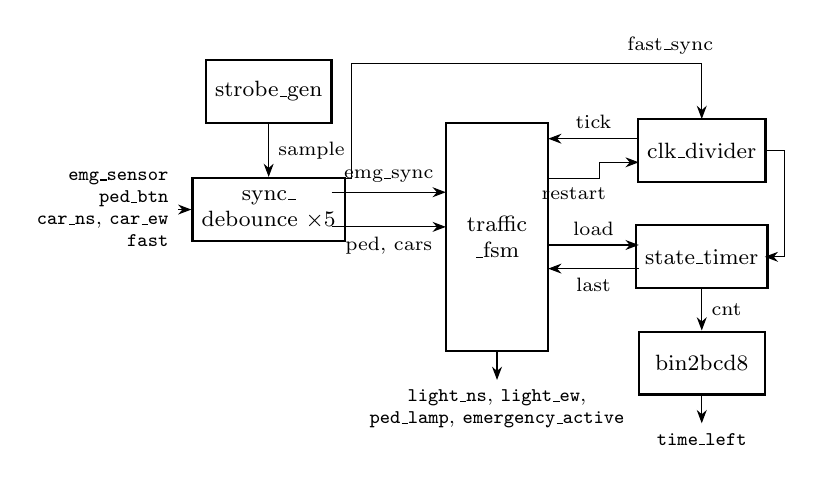
\begin{tikzpicture}[x=1cm,y=1cm]
  \node[blk, minimum width=15mm] (strobe) at (2.5,2.1) {strobe\_gen};
  \node[blk, minimum width=15mm] (db) at (2.5,0.6) {sync\_\\debounce $\times$5};
  \node[blk, minimum width=13mm, minimum height=29mm] (fsm) at (5.4,0.25) {traffic\\\_fsm};
  \node[blk, minimum width=16mm] (div) at (8.0,1.35) {clk\_divider};
  \node[blk, minimum width=16mm] (tim) at (8.0,0.0) {state\_timer};
  \node[blk, minimum width=16mm] (bcd) at (8.0,-1.35) {bin2bcd8};
  \node[sig, align=right, anchor=east] (in) at (1.35,0.6)
       {\code{emg\_sensor}\\\code{ped\_btn}\\\code{car\_ns}, \code{car\_ew}\\\code{fast}};
  \draw[->] (in) -- (db);
  \draw[->] (strobe) -- node[sig, right] {sample} (db);
  \draw[->] (3.3,0.82) -- node[sig, above] {emg\_sync} (4.75,0.82);
  \draw[->] (3.3,0.38) -- node[sig, below] {ped, cars} (4.75,0.38);
  \draw[->] (3.3,1.0) -- (3.55,1.0) |- (7.2,2.45) -| node[sig, pos=0.25, above] {fast\_sync} (8.0,1.75);
  \draw[->] (7.2,1.5) -- node[sig, above] {tick} (6.05,1.5);
  \draw[->] (6.05,1.0) -- node[sig, below] {restart} (6.7,1.0) |- (7.2,1.2);
  \draw[->] (6.05,0.15) -- node[sig, above] {load} (7.2,0.15);
  \draw[<-] (6.05,-0.15) -- node[sig, below] {last} (7.2,-0.15);
  \draw[->] (8.8,1.35) -- (9.05,1.35) |- (8.8,0.0);
  \draw[->] (tim) -- node[sig, right] {cnt} (bcd);
  \draw[->] (bcd.south) -- ++(0,-0.35) node[sig, below] {\code{time\_left}};
  \draw[->] (fsm.south) -- ++(0,-0.35) node[sig, below, align=center]
       {\code{light\_ns}, \code{light\_ew},\\ \code{ped\_lamp}, \code{emergency\_active}};
\end{tikzpicture}}
\caption{Block diagram of \code{traffic\_top}. The FSM restarts the time base
whenever a phase starts (\code{restart} = \code{load}).}
\label{fig:block}
\end{figure}

\subsection{State machine}
The controller is the 9-state Moore machine of Fig.~\ref{fig:fsm} and
Table~\ref{tab:fsm}. With $\mathit{done} = \mathit{tick}\wedge(\mathit{cnt}=1)$,
the last tick of a phase, the priority in every state is
$\mathit{emg} > \mathit{done}\wedge\mathit{ext\_ok} > \mathit{done}\wedge\mathit{ped}
> \mathit{done}$. The green of a road is extended by one tick at a time while no
car waits on the other road, no pedestrian is waiting and fewer than
$T_{G,max}-T_G$ extensions were granted.

The emergency override follows four rules.
\begin{enumerate}
\item An emergency during a green ends the green at once, but through the full
      yellow: green never turns red directly. A yellow in progress is never cut.
\item Once all directions are red, the controller stays in \st{EMERGENCY}, without
      timeout, until the request is released, then spends $T_{RC}$ in
      \st{RECOVER} (all red).
\item The road that was stopped gives way: a flag \code{next\_ew}, set when
      \st{NS\_Y} is entered and cleared when \st{EW\_Y} is entered, chooses the
      green that follows \st{RECOVER} or \st{PED\_WALK}.
\item A pending pedestrian request survives the emergency and is served after
      \st{RECOVER}; an emergency during \st{PED\_WALK} ends the walk.
\end{enumerate}

\begin{figure}[t]
\centering
\resizebox{\columnwidth}{!}{%
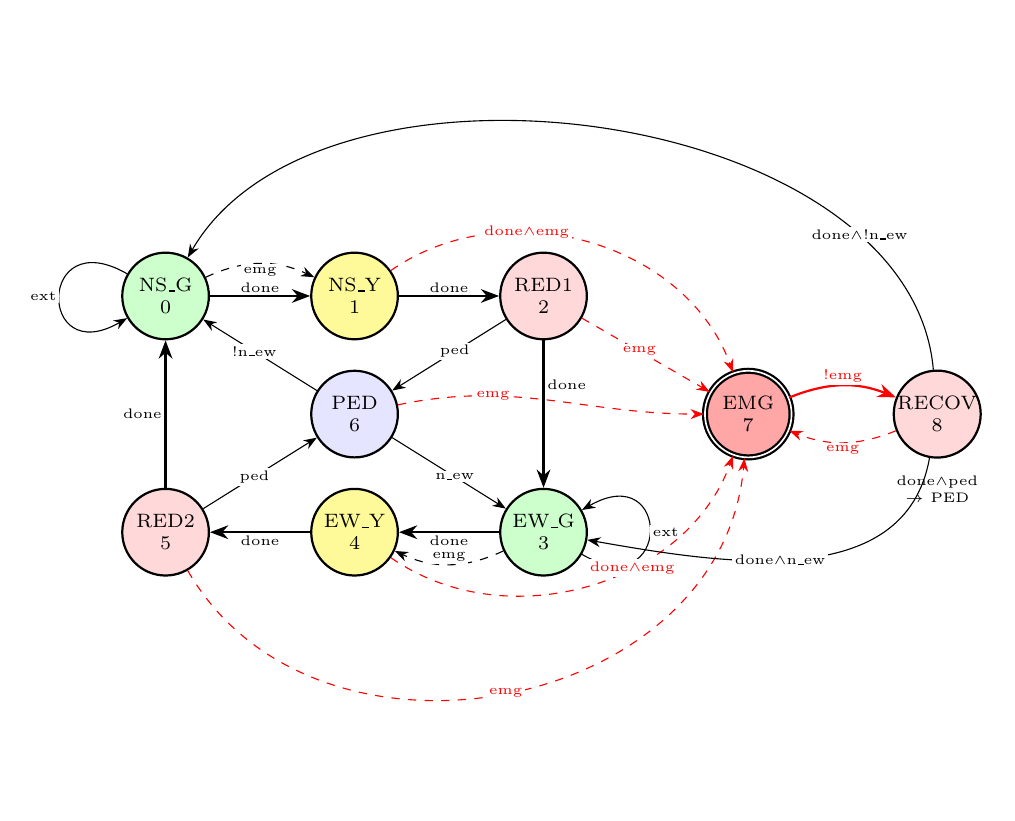
\begin{tikzpicture}[x=1cm,y=1cm,>=Stealth]
  \node[sm, fill=green!20] (nsg) at (0,3)   {NS\_G\\0};
  \node[sm, fill=yellow!40] (nsy) at (2.4,3) {NS\_Y\\1};
  \node[sm, fill=red!15] (r1)  at (4.8,3)   {RED1\\2};
  \node[sm, fill=green!20] (ewg) at (4.8,0) {EW\_G\\3};
  \node[sm, fill=yellow!40] (ewy) at (2.4,0) {EW\_Y\\4};
  \node[sm, fill=red!15] (r2)  at (0,0)     {RED2\\5};
  \node[sm, fill=blue!10] (ped) at (2.4,1.5) {PED\\6};
  \node[sm, fill=red!35, double] (emg) at (7.4,1.5) {EMG\\7};
  \node[sm, fill=red!15] (rec) at (9.8,1.5)  {RECOV\\8};
  % normal cycle
  \draw[->, thick] (nsg) -- node[lbl, above] {done} (nsy);
  \draw[->, thick] (nsy) -- node[lbl, above] {done} (r1);
  \draw[->, thick] (r1) -- node[lbl, right, pos=0.3] {done} (ewg);
  \draw[->, thick] (ewg) -- node[lbl, below] {done} (ewy);
  \draw[->, thick] (ewy) -- node[lbl, below] {done} (r2);
  \draw[->, thick] (r2) -- node[lbl, left] {done} (nsg);
  \draw[->] (nsg) to[out=150,in=210,looseness=6] node[lbl, left] {ext} (nsg);
  \draw[->] (ewg) to[out=-30,in=30,looseness=6] node[lbl, right] {ext} (ewg);
  \draw[->, dashed] (nsg) to[bend left=25] node[lbl, below] {emg} (nsy);
  \draw[->, dashed] (ewg) to[bend left=25] node[lbl, above] {emg} (ewy);
  % pedestrian
  \draw[->] (r1) -- node[lbl, pos=0.45] {ped} (ped);
  \draw[->] (r2) -- node[lbl, pos=0.45] {ped} (ped);
  \draw[->] (ped) -- node[lbl, pos=0.55] {!n\_ew} (nsg);
  \draw[->] (ped) -- node[lbl, pos=0.55] {n\_ew} (ewg);
  % emergency
  \draw[->, red, dashed] (nsy) to[out=35,in=110] node[lbl, pos=0.35] {done$\wedge$emg} (emg);
  \draw[->, red, dashed] (r1) -- node[lbl, pos=0.45] {emg} (emg);
  \draw[->, red, dashed] (ped) to[out=12,in=180] node[lbl, pos=0.3] {emg} (emg);
  \draw[->, red, dashed] (ewy) to[out=-35,in=-110] node[lbl, pos=0.62] {done$\wedge$emg} (emg);
  \draw[->, red, dashed] (r2) to[out=-60,in=-95,looseness=1.15] node[lbl, pos=0.5] {emg} (emg);
  \draw[->, red, thick] (emg) to[bend left=22] node[lbl, above] {!emg} (rec);
  \draw[->, red, dashed] (rec) to[bend left=22] node[lbl, below] {emg} (emg);
  \draw[->] (rec) to[out=-100,in=-10] node[lbl, pos=0.55] {done$\wedge$n\_ew} (ewg);
  \draw[->] (rec) to[out=95,in=60,looseness=0.9] node[lbl, pos=0.2] {done$\wedge$!n\_ew} (nsg);
  \node[font=\tiny, align=center] at (9.8,0.55) {done$\wedge$ped\\$\to$ PED};
\end{tikzpicture}}
\caption{State diagram. Black: normal cycle (thick), green extension (ext) and
pedestrian phase; dashed red: emergency arcs. n\_ew: \code{next\_ew}. Priority in
every state: emg, then extension, then pedestrian, then end of phase.}
\label{fig:fsm}
\end{figure}

\begin{table*}[t]
\centering
\caption{Transitions (priority from left to right) and phase lengths}
\label{tab:fsm}
\scriptsize
\setlength{\tabcolsep}{3pt}
\begin{tabular}{@{}l c c c l c@{}}
\toprule
State & NS & EW & walk & Next state & Ticks \\
\midrule
\st{NS\_G} (0) & G & R & 0 & emg $\to$ \st{NS\_Y}; done$\wedge$ext\_ok: stay 1 tick; done $\to$ \st{NS\_Y} & $T_G$ \\
\st{NS\_Y} (1) & Y & R & 0 & done $\to$ emg ? \st{EMG} : \st{RED1} & $T_Y$ \\
\st{RED1} (2) & R & R & 0 & emg $\to$ \st{EMG}; done $\to$ ped ? \st{PED} : \st{EW\_G} & $T_R$ \\
\st{EW\_G} (3) & R & G & 0 & as \st{NS\_G} with \code{car\_ns} & $T_G$ \\
\st{EW\_Y} (4) & R & Y & 0 & done $\to$ emg ? \st{EMG} : \st{RED2} & $T_Y$ \\
\st{RED2} (5) & R & R & 0 & emg $\to$ \st{EMG}; done $\to$ ped ? \st{PED} : \st{NS\_G} & $T_R$ \\
\st{PED\_WALK} (6) & R & R & 1 & emg $\to$ \st{EMG}; done $\to$ n\_ew ? \st{EW\_G} : \st{NS\_G} & $T_{WALK}$ \\
\st{EMERGENCY} (7) & R & R & 0 & !emg $\to$ \st{RECOVER} & -- \\
\st{RECOVER} (8) & R & R & 0 & emg $\to$ \st{EMG}; done $\to$ ped ? \st{PED} : n\_ew ? \st{EW\_G} : \st{NS\_G} & $T_{RC}$ \\
\bottomrule
\end{tabular}
\end{table*}

\subsection{Time base restarted at every phase}
The tick is not free-running. Whenever the state changes, the timer loads the
length of the new phase and \code{clk\_divider} clears its count, so the first
tick of the phase comes exactly $\mathit{DIV}$ cycles later and a phase of $T$
ticks lasts exactly $T\cdot\mathit{DIV}$ cycles. For a phase that starts on a
tick (the end of the previous phase) this changes nothing: the divider was
wrapping to zero anyway. It matters for the phases that start between two ticks,
which are exactly the emergency ones: with a free-running divider, a yellow forced
by an emergency lasts between $(T_Y-1)\mathit{DIV}+1$ and $T_Y\cdot\mathit{DIV}$
cycles, i.e.\ between 2 and 3~s on the board. Mutant M6 in
Section~\ref{sec:verif} removes the restart and is caught by the yellow-length
property.

The worst delay from the (debounced) emergency request to all red is then
\begin{equation}
L = T_Y\cdot\mathit{DIV} + 1 \text{ cycles},
\label{eq:lat}
\end{equation}
reached when the request arrives during a green: one cycle to enter the yellow,
then the full yellow. On the board the input path adds two synchronizer cycles and
at most three debounce samples (15~ms), about 3.015~s in total.

% =============================================================================
\section{RTL Implementation}\label{sec:rtl}

The RTL consists of seven SystemVerilog modules: \code{strobe\_gen},
\code{sync\_debounce}, \code{clk\_divider}, \code{state\_timer},
\code{traffic\_fsm}, \code{bin2bcd8} and \code{traffic\_top}. The same files are
simulated with Icarus Verilog~0.9.7~\cite{icarus}, ModelSim-Altera~\MsimVersion{}
and synthesized with Quartus~II, which fixes the coding rules:
\begin{itemize}
\item state codes are \code{localparam} constants, not an \code{enum} (Icarus
      0.9.7 has no \code{enum}; Quartus still extracts the state
      machine~\cite{quartus13});
\item each \code{always\_comb} assigns a default to every output, so no latch is
      inferred; registers use \code{always\_ff} with non-blocking assignments and
      an asynchronous active-low reset~\cite{cummings03};
\item every net between two instances and every continuous assignment is a
      \code{wire}: the down-converter used for Icarus~0.9.7 turns \code{logic}
      into \code{reg}, which cannot be driven by an instance output;
\item an expression that becomes a constant for some parameter value (the strobe
      when $\code{DB\_DIV}=1$) is a continuous assignment, because the
      \code{always @*} made from an \code{always\_comb} would never execute.
\end{itemize}

The next-state logic (Listing~\ref{lst:fsm}) is one \code{always\_comb} block with
a \code{unique case}; the timer load is \code{load = (next\_state != state)} and
the lights are registered from \code{next\_state}, so they change on the same
clock edge as the state register and cannot glitch. \code{state\_dbg} is a decode
of the state, never the state register itself, so that the synthesis tool remains
free to re-encode it.

\lstinputlisting[float=t, firstline=88, lastline=123, caption={Next-state logic
of \code{traffic\_fsm.sv}}, label=lst:fsm]{../rtl/traffic_fsm.sv}

\code{clk\_divider} decodes the tick one cycle early ($\mathit{cnt} =
\mathit{DIV}-2$) and registers it. The waveform is identical to the
combinational decode ($\mathit{cnt} = \mathit{DIV}-1$), but the 26-bit comparison
no longer lies on the path to the FSM. \code{bin2bcd8} uses double dabble
(\LEBcd{} logic elements): a first version built as a loop of subtract-ten
comparisons was several times larger and alone pushed the design above the
300-element target. The debouncer passes a change only
after three equal samples: glitches shorter than 10~ms never reach the FSM on the
board.

% =============================================================================
\section{Verification}\label{sec:verif}

\begin{figure}[t]
\centering
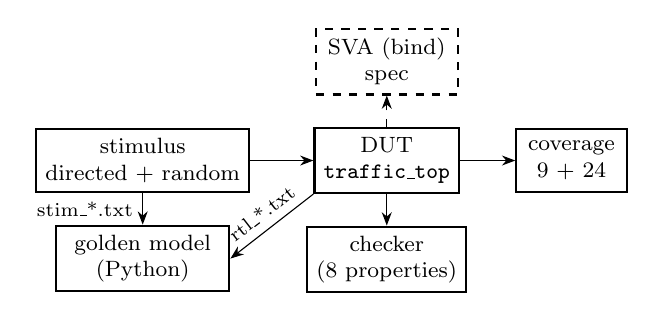
\begin{tikzpicture}[node distance=3mm and 5mm]
  \node[blk, minimum width=22mm] (stim) {stimulus\\directed + random};
  \node[blk, right=8mm of stim, minimum width=18mm] (dut) {DUT\\\code{traffic\_top}};
  \node[blk, below=4mm of dut, minimum width=18mm] (chk) {checker\\(8 properties)};
  \node[blk, above=4mm of dut, minimum width=18mm, dashed] (sva) {SVA (bind)\\spec};
  \node[blk, right=7mm of dut, minimum width=14mm] (cov) {coverage\\9 + 24};
  \node[blk, below=4mm of stim, minimum width=22mm] (gold) {golden model\\(Python)};
  \draw[->] (stim) -- (dut);
  \draw[->] (dut) -- (chk);
  \draw[->, dashed] (dut) -- (sva);
  \draw[->] (dut) -- (cov);
  \draw[->] (stim) -- node[sig, left] {stim\_*.txt} (gold);
  \draw[->] (dut.south west) -- node[sig, above, sloped] {rtl\_*.txt} (gold.east);
\end{tikzpicture}
\caption{Verification environment (\code{traffic\_tb.sv}).}
\label{fig:tb}
\end{figure}

\subsection{Environment}
Fig.~\ref{fig:tb} shows the testbench. It drives \code{traffic\_top} with
$\code{TICK\_DIV}=4$, $\code{FAST\_DIV}=2$ and $\code{DB\_DIV}=1$; the inputs
change on falling clock edges. At every rising edge it writes the inputs and the
outputs to two text files, observes the state transitions for coverage and feeds
the checker. One run has two phases:
\begin{enumerate}
\item 18 directed tests (Table~\ref{tab:tests}), each started from a reset, with
      \DirChecks{} checks on the order of the states, the length of each phase in
      cycles, \code{time\_left} at the start of each phase and the flags
      (\DirCycles{} cycles);
\item \RandomCycles{} constrained-random cycles: an emergency in 1 of 400
      cycles held 5 to 60 cycles, a button press in 1 of 150, a 1- or 2-cycle
      glitch on one input in 1 of 50, a car sensor change in 1 of 80, a change of
      \code{fast} in 1 of 4000 and a reset in 1 of 5000 cycles.
\end{enumerate}
The flow runs seeds \SimSeeds{}: \SimCyclesAll{} cycles in total. All random
numbers of a cycle are drawn before they are used: SystemVerilog short-circuits
\code{\&\&}, so a \code{\$random} call inside a condition is skipped by ModelSim
but not by Icarus~0.9.7, and the two simulators would otherwise see different
stimuli. With this, both produce the same input and output trace, cycle for
cycle.

\begin{table}[t]
\centering
\caption{Directed tests}
\label{tab:tests}
\scriptsize
\setlength{\tabcolsep}{3pt}
\begin{tabular}{@{}l p{3.5cm} p{3.6cm}@{}}
\toprule
\# & Scenario & Checked \\
\midrule
T1 & two normal cycles & 10-3-1-10-3-1 ticks, 28 per cycle \\
T2 & button in \st{NS\_Y} & \st{PED\_WALK} after \st{RED1}, then \st{EW\_G} \\
T3 & button held / pressed 3 times & one \st{PED\_WALK} only \\
T4 & button in \st{PED\_WALK} & ignored \\
T5 & emergency in \st{NS\_G} & full yellow, \st{EMG}, \st{RECOVER}, \st{EW\_G} \\
T6 & emergency in \st{NS\_Y} & yellow not cut, then \st{EMG} \\
T7 & emergency in \st{PED\_WALK} & \st{EMG} at once, walk lamp off \\
T8 & emergency + button & \st{PED\_WALK} served after \st{RECOVER} \\
T9 & emergency again in \st{RECOVER} & back to \st{EMG} \\
T10 & reset in a phase & \st{NS\_G}, $T_G$ at once (asynchronous) \\
T11 & 1-, 2-cycle glitches & filtered \\
T12 & 3-cycle pulses & accepted \\
T13 & no car on the other road & green of 15 ticks, both roads \\
T14 & car arrives in an extension & green ends at the next tick \\
T15 & \code{fast} = 1 & every phase twice as short \\
T16 & emergency for 2000 cycles & all red, no timeout \\
T17 & emergency at each tick offset & yellow and \st{RECOVER} exact \\
T18 & emergency in \st{RED1}, \st{EW\_G}, \st{RED2} & coverage of the remaining arcs \\
\bottomrule
\end{tabular}
\end{table}

\subsection{Golden model}
\code{model/golden.py} is a cycle-accurate model of the whole path (strobe,
synchronizers, debouncers, divider with restart, timer, FSM, BCD), written from
the specification of Section~\ref{sec:arch}, not from the RTL. It replays the
stimulus file and compares its prediction of the state, both lights, the walk lamp,
\code{time\_left} and \code{emergency\_active} with the RTL trace at every cycle.
For the three seeds it agrees on all \GoldenCycles{} cycles, with no mismatch.

\subsection{Properties}
Eight properties are written as SystemVerilog concurrent assertions~\cite{sv17} in
\code{traffic\_sva.sv}, bound to \code{traffic\_top}; the first three come from the
proposal:
\begin{itemize}
\item \code{a\_safe}: never green on both roads;
\item \code{a\_emg}: \code{\$rose(emg\_sync) |-> \#\#[1:3] emergency\_active};
\item \code{a\_yel}: \code{\$fell(green) |-> yellow}, for each road;
\item \code{a\_onehot}, \code{a\_ped}: one lamp per road; walk lamp only with
      both roads red;
\item \code{a\_allred}: \code{emg\_sync} held for more than $L$ cycles
      (\ref{eq:lat}) $\Rightarrow$ all red;
\item \code{a\_gmax}: a green lasts at most $T_{G,max}\cdot\mathit{DIV}$ cycles;
\item \code{a\_ylen}: a yellow lasts exactly $T_Y\cdot\mathit{DIV}$ cycles.
\end{itemize}
ModelSim-Altera Starter Edition compiles the SVA file but does not execute
concurrent assertions (warning \code{vsim-8311}: ``supported only in Questasim''),
and Icarus does not parse them. The results therefore come from
\code{traffic\_checker.sv}, which implements the same properties with cycle
counters and immediate assertions and runs on both simulators. Table~\ref{tab:props}
shows how often each property was triggered (its antecedent was true): none of
them passes vacuously.

\begin{table}[t]
\centering
\caption{Properties over the three seeds}
\label{tab:props}
\footnotesize
\begin{tabular}{@{}l r r@{}}
\toprule
Property & Triggered & Violations \\
\midrule
\code{a\_safe}   & \HitSafe   & 0 \\
\code{a\_emg}    & \HitEmg    & 0 \\
\code{a\_yel}    & \HitYel    & 0 \\
\code{a\_onehot} & \HitOnehot & 0 \\
\code{a\_ped}    & \HitPed    & 0 \\
\code{a\_allred} & \HitAllred & 0 \\
\code{a\_gmax}   & \HitGmax   & 0 \\
\code{a\_ylen}   & \HitYlen   & 0 \\
\bottomrule
\end{tabular}
\end{table}

\subsection{Coverage}
The testbench counts the entries into each state and the transitions taken,
distinguished by their condition: 24 arcs, e.g.\ \st{NS\_G}$\to$\st{NS\_Y} by
emergency and by end of phase are two arcs. With the three seeds all 9 states and
all 24 arcs are covered; the least frequent arc, \ArcMinName, is taken \ArcMin{}
times. An emergency request rising inside the 4-cycle \st{RED1}
phase is rare under random stimulus (the debouncer alone takes 5 cycles), which
is why T18 targets it.

\subsection{Mutation}
To check that the environment detects errors, six mutants of the RTL are
simulated with seed~1 (Table~\ref{tab:mut}). Every mutant is caught by the
directed tests, by the checker and by the golden model; M1 and M5 violate the two
safety properties of the proposal, and M6, the divider without restart, is caught
by \code{a\_ylen} and by test T17.

\begin{table}[t]
\centering
\caption{Mutants (seed 1): directed errors, checker violations, golden model mismatches}
\label{tab:mut}
\scriptsize
\setlength{\tabcolsep}{2.5pt}
\begin{tabular}{@{}l p{3.0cm} r r l r@{}}
\toprule
& Mutation & Dir. & Chk. & Properties & Golden \\
\midrule
M1 & green $\to$ \st{EMG} without yellow & \MutErrA & \MutViolA & \MutPropsA & \MutGoldA \\
M2 & 2-sample debouncer & \MutErrB & \MutViolB & \MutPropsB & \MutGoldB \\
M3 & request not latched & \MutErrC & \MutViolC & \MutPropsC & \MutGoldC \\
M4 & \st{NS\_Y} $\to$ \st{EW\_G} (no \st{RED1}) & \MutErrD & \MutViolD & \MutPropsD & \MutGoldD \\
M5 & EW green with \st{NS\_G} & \MutErrE & \MutViolE & \MutPropsE & \MutGoldE \\
M6 & no divider restart & \MutErrF & \MutViolF & \MutPropsF & \MutGoldF \\
\bottomrule
\end{tabular}
\end{table}

\subsection{Waveforms}
Fig.~\ref{fig:wave} is drawn from the VCD file of test T5: the switch rises at
\ding{172}, the debounced request reaches the FSM at the \WaveDbLat{}th rising
edge and the green ends; the yellow \ding{173} lasts \WaveYellow{} cycles (3
ticks) although it started between two ticks; at \ding{174} every lamp is red and
\code{time\_left} shows 00; after the release \ding{175}, \st{RECOVER}
\ding{176} lasts \WaveRecover{} cycles and the EW road, which was not stopped,
gets the green. Fig.~\ref{fig:gtk} shows the same test and T2 in GTKWave.

\begin{figure*}[t]
\centering
\resizebox{\textwidth}{!}{% Generated by make_figures.py from traffic_tb.vcd (T5) - do not edit.
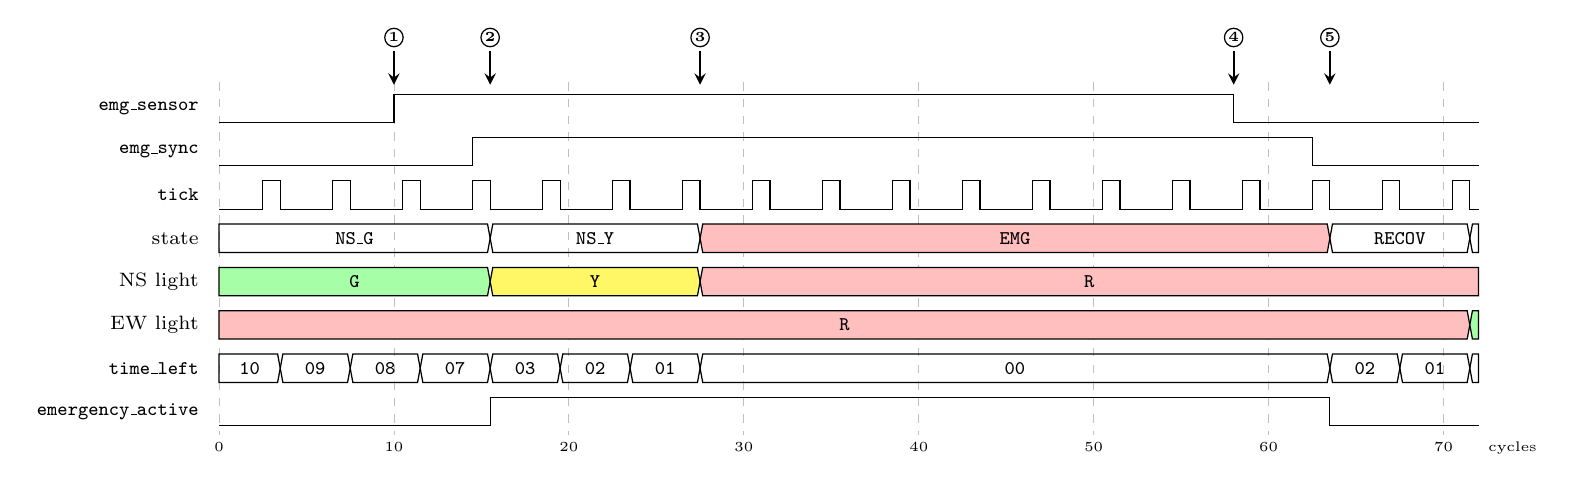
\begin{tikzpicture}[x=0.02222cm,y=1cm,font=\scriptsize,line width=0.45pt]
\draw[black!25,dashed,line width=0.3pt] (0.0,0.15) -- (0.0,-4.33);
\node[below=-1pt,font=\tiny] at (0.0,-4.33) {0};
\draw[black!25,dashed,line width=0.3pt] (100.0,0.15) -- (100.0,-4.33);
\node[below=-1pt,font=\tiny] at (100.0,-4.33) {10};
\draw[black!25,dashed,line width=0.3pt] (200.0,0.15) -- (200.0,-4.33);
\node[below=-1pt,font=\tiny] at (200.0,-4.33) {20};
\draw[black!25,dashed,line width=0.3pt] (300.0,0.15) -- (300.0,-4.33);
\node[below=-1pt,font=\tiny] at (300.0,-4.33) {30};
\draw[black!25,dashed,line width=0.3pt] (400.0,0.15) -- (400.0,-4.33);
\node[below=-1pt,font=\tiny] at (400.0,-4.33) {40};
\draw[black!25,dashed,line width=0.3pt] (500.0,0.15) -- (500.0,-4.33);
\node[below=-1pt,font=\tiny] at (500.0,-4.33) {50};
\draw[black!25,dashed,line width=0.3pt] (600.0,0.15) -- (600.0,-4.33);
\node[below=-1pt,font=\tiny] at (600.0,-4.33) {60};
\draw[black!25,dashed,line width=0.3pt] (700.0,0.15) -- (700.0,-4.33);
\node[below=-1pt,font=\tiny] at (700.0,-4.33) {70};
\node[below=-1pt,font=\tiny,anchor=north west] at (720.0,-4.33) {cycles};
\node[anchor=east] at (-6,-0.18) {\code{emg\_sensor}};
\draw (0.00,-0.36) -- (100.00,-0.36) -- (100.00,0.00) -- (580.00,0.00) -- (580.00,-0.36) -- (720.00,-0.36);
\node[anchor=east] at (-6,-0.73) {\code{emg\_sync}};
\draw (0.00,-0.91) -- (145.00,-0.91) -- (145.00,-0.55) -- (625.00,-0.55) -- (625.00,-0.91) -- (720.00,-0.91);
\node[anchor=east] at (-6,-1.28) {\code{tick}};
\draw (0.00,-1.46) -- (25.00,-1.46) -- (25.00,-1.10) -- (35.00,-1.10) -- (35.00,-1.46) -- (65.00,-1.46) -- (65.00,-1.10) -- (75.00,-1.10) -- (75.00,-1.46) -- (105.00,-1.46) -- (105.00,-1.10) -- (115.00,-1.10) -- (115.00,-1.46) -- (145.00,-1.46) -- (145.00,-1.10) -- (155.00,-1.10) -- (155.00,-1.46) -- (185.00,-1.46) -- (185.00,-1.10) -- (195.00,-1.10) -- (195.00,-1.46) -- (225.00,-1.46) -- (225.00,-1.10) -- (235.00,-1.10) -- (235.00,-1.46) -- (265.00,-1.46) -- (265.00,-1.10) -- (275.00,-1.10) -- (275.00,-1.46) -- (305.00,-1.46) -- (305.00,-1.10) -- (315.00,-1.10) -- (315.00,-1.46) -- (345.00,-1.46) -- (345.00,-1.10) -- (355.00,-1.10) -- (355.00,-1.46) -- (385.00,-1.46) -- (385.00,-1.10) -- (395.00,-1.10) -- (395.00,-1.46) -- (425.00,-1.46) -- (425.00,-1.10) -- (435.00,-1.10) -- (435.00,-1.46) -- (465.00,-1.46) -- (465.00,-1.10) -- (475.00,-1.10) -- (475.00,-1.46) -- (505.00,-1.46) -- (505.00,-1.10) -- (515.00,-1.10) -- (515.00,-1.46) -- (545.00,-1.46) -- (545.00,-1.10) -- (555.00,-1.10) -- (555.00,-1.46) -- (585.00,-1.46) -- (585.00,-1.10) -- (595.00,-1.10) -- (595.00,-1.46) -- (625.00,-1.46) -- (625.00,-1.10) -- (635.00,-1.10) -- (635.00,-1.46) -- (665.00,-1.46) -- (665.00,-1.10) -- (675.00,-1.10) -- (675.00,-1.46) -- (705.00,-1.46) -- (705.00,-1.10) -- (715.00,-1.10) -- (715.00,-1.46) -- (720.00,-1.46);
\node[anchor=east] at (-6,-1.83) {state};
\draw[] (0.00,-1.83) -- (0.00,-1.65) -- (153.50,-1.65) -- (155.00,-1.83) -- (153.50,-2.01) -- (0.00,-2.01) -- cycle;
\node at (77.50,-1.83) {\code{NS\_G}};
\draw[] (155.00,-1.83) -- (156.50,-1.65) -- (273.50,-1.65) -- (275.00,-1.83) -- (273.50,-2.01) -- (156.50,-2.01) -- cycle;
\node at (215.00,-1.83) {\code{NS\_Y}};
\draw[fill=red!25] (275.00,-1.83) -- (276.50,-1.65) -- (633.50,-1.65) -- (635.00,-1.83) -- (633.50,-2.01) -- (276.50,-2.01) -- cycle;
\node at (455.00,-1.83) {\code{EMG}};
\draw[] (635.00,-1.83) -- (636.50,-1.65) -- (713.50,-1.65) -- (715.00,-1.83) -- (713.50,-2.01) -- (636.50,-2.01) -- cycle;
\node at (675.00,-1.83) {\code{RECOV}};
\draw[] (715.00,-1.83) -- (716.50,-1.65) -- (720.00,-1.65) -- (720.00,-1.83) -- (720.00,-2.01) -- (716.50,-2.01) -- cycle;
\node[anchor=east] at (-6,-2.38) {NS light};
\draw[fill=green!35] (0.00,-2.38) -- (0.00,-2.20) -- (153.50,-2.20) -- (155.00,-2.38) -- (153.50,-2.56) -- (0.00,-2.56) -- cycle;
\node at (77.50,-2.38) {\code{G}};
\draw[fill=yellow!60] (155.00,-2.38) -- (156.50,-2.20) -- (273.50,-2.20) -- (275.00,-2.38) -- (273.50,-2.56) -- (156.50,-2.56) -- cycle;
\node at (215.00,-2.38) {\code{Y}};
\draw[fill=red!25] (275.00,-2.38) -- (276.50,-2.20) -- (720.00,-2.20) -- (720.00,-2.38) -- (720.00,-2.56) -- (276.50,-2.56) -- cycle;
\node at (497.50,-2.38) {\code{R}};
\node[anchor=east] at (-6,-2.93) {EW light};
\draw[fill=red!25] (0.00,-2.93) -- (0.00,-2.75) -- (713.50,-2.75) -- (715.00,-2.93) -- (713.50,-3.11) -- (0.00,-3.11) -- cycle;
\node at (357.50,-2.93) {\code{R}};
\draw[fill=green!35] (715.00,-2.93) -- (716.50,-2.75) -- (720.00,-2.75) -- (720.00,-2.93) -- (720.00,-3.11) -- (716.50,-3.11) -- cycle;
\node[anchor=east] at (-6,-3.48) {\code{time\_left}};
\draw[] (0.00,-3.48) -- (0.00,-3.30) -- (33.50,-3.30) -- (35.00,-3.48) -- (33.50,-3.66) -- (0.00,-3.66) -- cycle;
\node at (17.50,-3.48) {\code{10}};
\draw[] (35.00,-3.48) -- (36.50,-3.30) -- (73.50,-3.30) -- (75.00,-3.48) -- (73.50,-3.66) -- (36.50,-3.66) -- cycle;
\node at (55.00,-3.48) {\code{09}};
\draw[] (75.00,-3.48) -- (76.50,-3.30) -- (113.50,-3.30) -- (115.00,-3.48) -- (113.50,-3.66) -- (76.50,-3.66) -- cycle;
\node at (95.00,-3.48) {\code{08}};
\draw[] (115.00,-3.48) -- (116.50,-3.30) -- (153.50,-3.30) -- (155.00,-3.48) -- (153.50,-3.66) -- (116.50,-3.66) -- cycle;
\node at (135.00,-3.48) {\code{07}};
\draw[] (155.00,-3.48) -- (156.50,-3.30) -- (193.50,-3.30) -- (195.00,-3.48) -- (193.50,-3.66) -- (156.50,-3.66) -- cycle;
\node at (175.00,-3.48) {\code{03}};
\draw[] (195.00,-3.48) -- (196.50,-3.30) -- (233.50,-3.30) -- (235.00,-3.48) -- (233.50,-3.66) -- (196.50,-3.66) -- cycle;
\node at (215.00,-3.48) {\code{02}};
\draw[] (235.00,-3.48) -- (236.50,-3.30) -- (273.50,-3.30) -- (275.00,-3.48) -- (273.50,-3.66) -- (236.50,-3.66) -- cycle;
\node at (255.00,-3.48) {\code{01}};
\draw[] (275.00,-3.48) -- (276.50,-3.30) -- (633.50,-3.30) -- (635.00,-3.48) -- (633.50,-3.66) -- (276.50,-3.66) -- cycle;
\node at (455.00,-3.48) {\code{00}};
\draw[] (635.00,-3.48) -- (636.50,-3.30) -- (673.50,-3.30) -- (675.00,-3.48) -- (673.50,-3.66) -- (636.50,-3.66) -- cycle;
\node at (655.00,-3.48) {\code{02}};
\draw[] (675.00,-3.48) -- (676.50,-3.30) -- (713.50,-3.30) -- (715.00,-3.48) -- (713.50,-3.66) -- (676.50,-3.66) -- cycle;
\node at (695.00,-3.48) {\code{01}};
\draw[] (715.00,-3.48) -- (716.50,-3.30) -- (720.00,-3.30) -- (720.00,-3.48) -- (720.00,-3.66) -- (716.50,-3.66) -- cycle;
\node[anchor=east] at (-6,-4.03) {\code{emergency\_active}};
\draw (0.00,-4.21) -- (155.00,-4.21) -- (155.00,-3.85) -- (635.00,-3.85) -- (635.00,-4.21) -- (720.00,-4.21);
\draw[->,>=stealth,thick] (100.0,0.55) -- (100.0,0.12);
\node[circle,draw,inner sep=0.6pt,font=\tiny\bfseries] at (100.0,0.72) {1};
\draw[->,>=stealth,thick] (155.0,0.55) -- (155.0,0.12);
\node[circle,draw,inner sep=0.6pt,font=\tiny\bfseries] at (155.0,0.72) {2};
\draw[->,>=stealth,thick] (275.0,0.55) -- (275.0,0.12);
\node[circle,draw,inner sep=0.6pt,font=\tiny\bfseries] at (275.0,0.72) {3};
\draw[->,>=stealth,thick] (580.0,0.55) -- (580.0,0.12);
\node[circle,draw,inner sep=0.6pt,font=\tiny\bfseries] at (580.0,0.72) {4};
\draw[->,>=stealth,thick] (635.0,0.55) -- (635.0,0.12);
\node[circle,draw,inner sep=0.6pt,font=\tiny\bfseries] at (635.0,0.72) {5};
\end{tikzpicture}
}
\caption{Test T5 (emergency during \st{NS\_G}), drawn from the VCD file. One tick
is 4 clock cycles. Numbered events are explained in the text.}
\label{fig:wave}
\end{figure*}

\begin{figure*}[t]
\centering
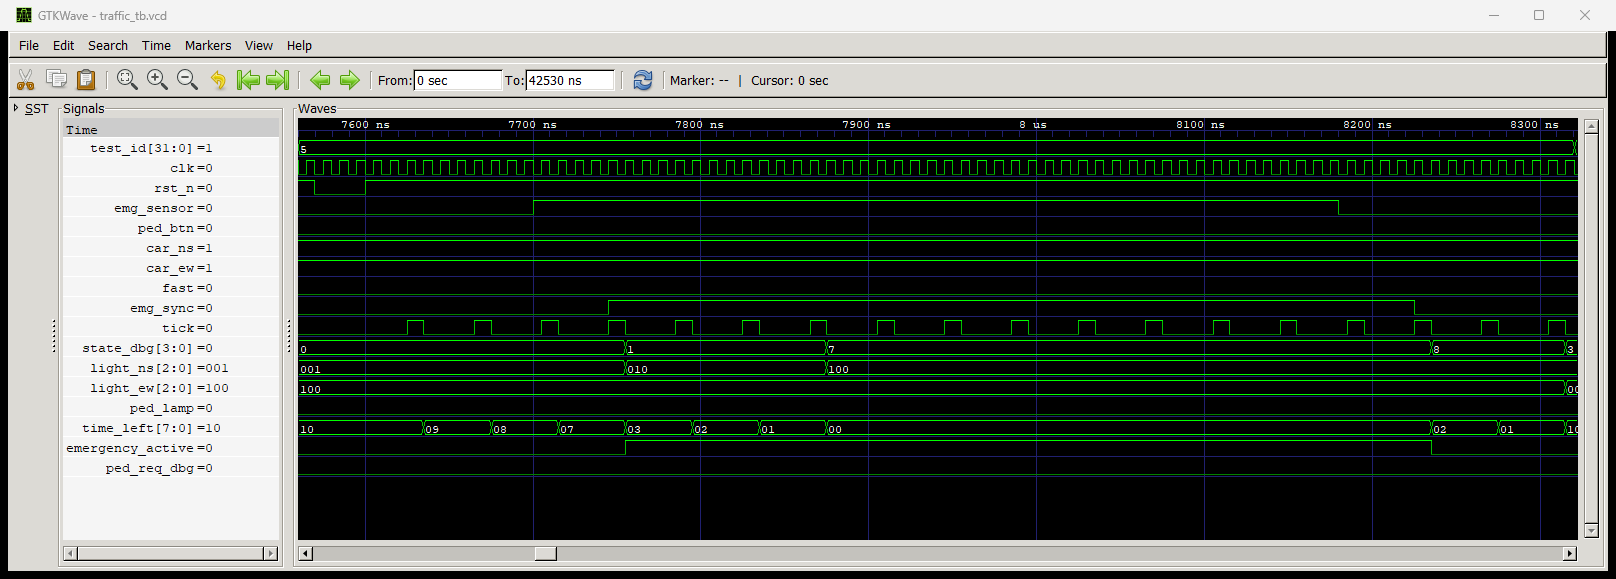
\includegraphics[width=0.88\textwidth]{gtkwave_T5.png}\\[2pt]
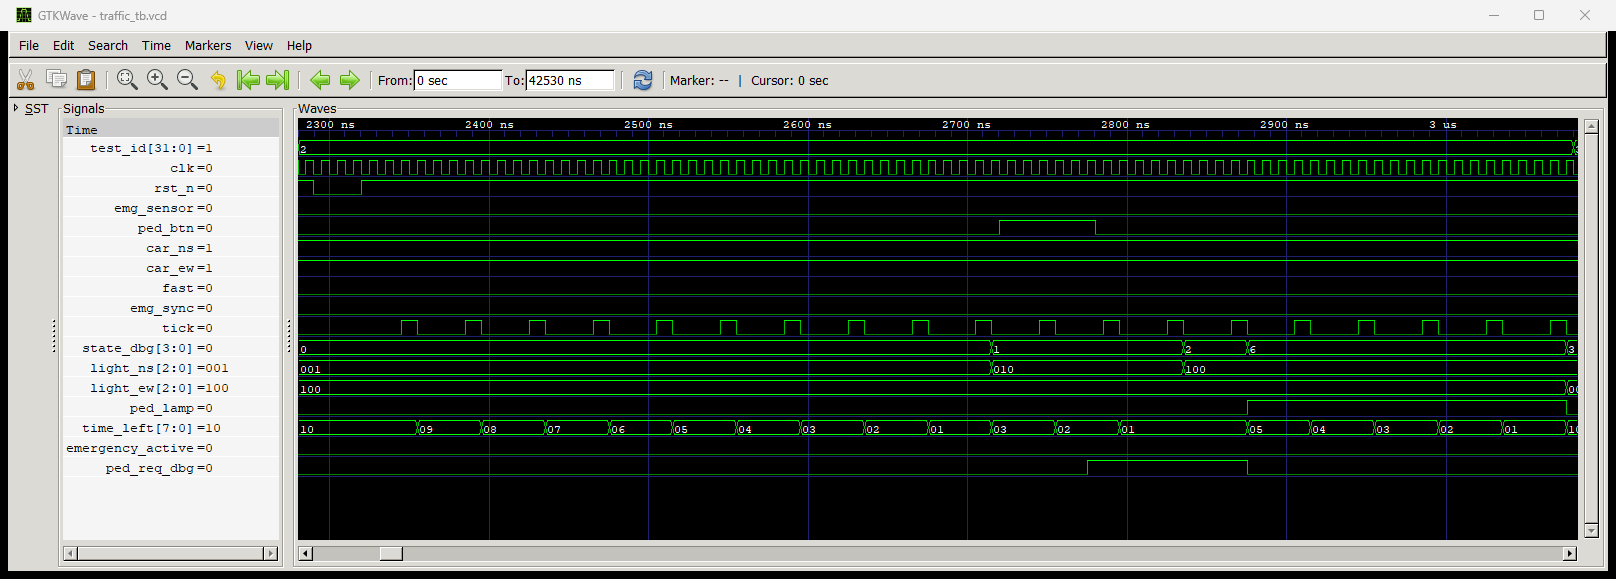
\includegraphics[width=0.88\textwidth]{gtkwave_T2.png}
\caption{GTKWave: test T5 (top, emergency during \st{NS\_G}) and test T2
(bottom, button pressed during \st{NS\_Y}: \code{ped\_req} is latched,
\st{PED\_WALK} follows \st{RED1}).}
\label{fig:gtk}
\end{figure*}

% =============================================================================
\section{Synthesis and Timing}\label{sec:synth}

The single Quartus~II project \code{de2\_traffic} targets the EP2C35F672C6 with
the board parameters. The SDC constrains the 50~MHz clock (20~ns); the switches,
buttons and displays are asynchronous or read by a human, so their paths are
declared false paths. \code{derive\_clock\_uncertainty} is not used: Quartus
reports that the Cyclone~II family does not support jitter analysis. Cyclone~II
has two timing models, slow and fast~\cite{cyclone2}; all frequencies below are from the slow
model.

\subsection{State encoding}
The same project was compiled three times with \code{STATE\_MACHINE\_PROCESSING}
set to sequential (binary), Gray and one-hot (Table~\ref{tab:enc}). Quartus
extracted the state machine every time; the map report confirms the encoding and
lists \BitsBin, \BitsGray{} and \BitsHot{} state bits. One-hot is the smallest and the fastest here: the
decoding of the state into lights, timer value and \code{state\_dbg} becomes a
few OR gates, which more than pays for the extra flip-flops. It is the
encoding of the final version (Quartus also chooses one-hot when the setting is
\code{AUTO}). None of the builds has a latch or a critical warning.

\begin{table}[t]
\centering
\caption{State encodings (complete design)}
\label{tab:enc}
\footnotesize
\begin{tabular}{@{}l r r r r@{}}
\toprule
Encoding & State bits & LE & Registers & Fmax (MHz) \\
\midrule
Binary  & \BitsBin  & \LEBin  & \FFBin  & \FmaxBin \\
Gray    & \BitsGray & \LEGray & \FFGray & \FmaxGray \\
One-hot & \BitsHot  & \LEHot  & \FFHot  & \FmaxHot \\
\bottomrule
\end{tabular}
\end{table}

\subsection{Resources and timing of the final version}
Table~\ref{tab:res} splits the \LEtotal{} logic elements of the one-hot build by
module. The 26-bit divider, the 18-bit debounce strobe and the 8-bit timer are
counters; the FSM itself takes \LEFsm{} logic elements. No memory block is used.
The slow-model Fmax is \FmaxSlow~MHz (fast model \FmaxFast~MHz). Checked against a
10~ns clock, the same fit has a setup slack of \SlackTen~ns, which confirms the
100~MHz target. The critical path, \CritDelay~ns, goes from the timer
(\CritFrom) through $\mathit{cnt}=1$, the next-state logic and the load
multiplexer back to the timer (\CritTo); thanks to the registered tick, the
26-bit divider comparison is not on it. The other slacks at 20~ns are positive:
setup \SlackSetup~ns, hold \SlackHold~ns, recovery \SlackRecovery~ns and removal
\SlackRemoval~ns.

\begin{table}[t]
\centering
\caption{Resources of the final version (one-hot)}
\label{tab:res}
\footnotesize
\begin{tabular}{@{}l r r@{}}
\toprule
Module & LE & Registers \\
\midrule
\code{traffic\_fsm} & \LEFsm & \FFFsm \\
\code{clk\_divider} & \LEDiv & \FFDiv \\
\code{strobe\_gen} & \LEStrobe & \FFStrobe \\
\code{state\_timer} & \LETimer & \FFTimer \\
\code{bin2bcd8} & \LEBcd & \FFBcd \\
\code{sync\_debounce} (each of 5) & \LEDb & \FFDb \\
\code{de2\_top} (displays, reset, heartbeat) & \LEtopOwn & \FFtopOwn \\
\midrule
Total & \LEtotal & \NumRegisters \\
\bottomrule
\end{tabular}
\end{table}

% =============================================================================
\section{FPGA Implementation}\label{sec:fpga}

\subsection{Board wrapper}
\code{de2\_top} instantiates \code{traffic\_top} with $\code{TICK\_DIV} =
5\cdot10^{7}$, $\code{FAST\_DIV} = 5\cdot10^{6}$ and $\code{DB\_DIV} =
2.5\cdot10^{5}$: the RTL is the one that was simulated, only the parameters
differ. \code{KEY[0]} resets the design through a two-flip-flop synchronizer
(asynchronous assertion, synchronous release)~\cite{cummingsrst}. The DE2 has no yellow LED, so the
lights are also shown as letters (\code{r}, \code{y}, \code{G}) on two 7-segment
displays; a green LED toggles at every tick, since a 20~ns tick pulse would not be
visible. Table~\ref{tab:pins} gives the pins~\cite{de2}; \code{CLOCK\_50} enters
the global clock network (\ClockGlobal). The design uses \NumPins{} pins.

\begin{table}[t]
\centering
\caption{Use of the DE2 board}
\label{tab:pins}
\scriptsize
\setlength{\tabcolsep}{3pt}
\begin{tabular}{@{}l l l@{}}
\toprule
Function & DE2 resource & Pin \\
\midrule
Clock & \code{CLOCK\_50} & N2 \\
Reset & \code{KEY[0]} & G26 \\
Pedestrian button & \code{KEY[1]} & N23 \\
Emergency sensor & \code{SW[0]} & N25 \\
Car NS / EW & \code{SW[1]} / \code{SW[2]} & N26 / P25 \\
Fast mode & \code{SW[17]} & V2 \\
NS R / Y / G & \code{LEDR[0]} / \code{LEDG[1]} / \code{LEDG[0]} & AE23 / AF22 / AE22 \\
EW R / Y / G & \code{LEDR[2]} / \code{LEDG[3]} / \code{LEDG[2]} & AB21 / V18 / W19 \\
Walk / request / emergency & \code{LEDR[17]} / \code{[16]} / \code{[15]} & AD12 / AE12 / AE13 \\
Heartbeat & \code{LEDG[8]} & Y12 \\
\code{time\_left} & \code{HEX1}--\code{HEX0} & \\
NS / EW light letter & \code{HEX3} / \code{HEX2} & \\
State number & \code{HEX4} & \\
\bottomrule
\end{tabular}
\end{table}

\subsection{On-board test}
The \code{.sof} file is loaded through the on-board USB-Blaster (JTAG, RUN/PROG
switch on RUN). Table~\ref{tab:board} lists the nine scenarios of the
demonstration and Fig.~\ref{fig:board} the photographs.\verify{V2}

\begin{table}[t]
\centering
\caption{Scenarios on the board (SW[17] = 0, 1 tick = 1~s)}
\label{tab:board}
\scriptsize
\setlength{\tabcolsep}{2.5pt}
\begin{tabular}{@{}l p{2.35cm} p{4.6cm}@{}}
\toprule
\# & Action & Expected \\
\midrule
B1 & reset, \code{SW[1]}=\code{SW[2]}=1 & HEX4 0-1-2-3-4-5-0; HEX3--2 \code{Gr yr rr rG ry rr}; 10-3-1 s; never two greens \\
B2 & \code{KEY[1]} in \st{NS\_G} & LEDR16 on; after \st{RED1}: HEX4=6, LEDR17 on 5 s, then EW green \\
B3 & \code{KEY[1]} held & one walk phase only \\
B4 & \code{SW[0]}=1 in \st{NS\_G} & LEDR15 on at once; NS yellow 3 s; HEX4=7, all red, HEX1--0=00 \\
B5 & hold \code{SW[0]}, then release & all red without timeout; HEX4=8 for 2 s, then EW green \\
B6 & \code{SW[0]}=1 in \st{PED\_WALK} & walk lamp off at once, \st{EMG} \\
B7 & \code{SW[2]}=0, \code{SW[1]}=1 & NS green up to 15 s (01 held 5 s); \code{SW[2]}=1 ends it \\
B8 & \code{KEY[0]} in a phase & \st{NS\_G}, HEX1--0 = 10 at once \\
B9 & \code{SW[0]} toggled fast, left at 1 & every cut green goes through 3 s of yellow; never two greens; ends in \st{EMG} \\
\bottomrule
\end{tabular}
\end{table}

\begin{figure*}[t]
\centering
\begin{minipage}[t]{0.32\textwidth}\centering\boardphoto{1}{B1: normal cycle}\\[3pt]\scriptsize B1: normal cycle\end{minipage}\hfill
\begin{minipage}[t]{0.32\textwidth}\centering\boardphoto{2}{B2: pedestrian walk}\\[3pt]\scriptsize B2: walk phase\end{minipage}\hfill
\begin{minipage}[t]{0.32\textwidth}\centering\boardphoto{3}{B3: button held}\\[3pt]\scriptsize B3: button held\end{minipage}\\[4pt]
\begin{minipage}[t]{0.32\textwidth}\centering\boardphoto{4}{B4: emergency, yellow}\\[3pt]\scriptsize B4: emergency in a green\end{minipage}\hfill
\begin{minipage}[t]{0.32\textwidth}\centering\boardphoto{5}{B5: RECOVER}\\[3pt]\scriptsize B5: release, \st{RECOVER}\end{minipage}\hfill
\begin{minipage}[t]{0.32\textwidth}\centering\boardphoto{6}{B6: emergency in walk}\\[3pt]\scriptsize B6: emergency in \st{PED\_WALK}\end{minipage}\\[4pt]
\begin{minipage}[t]{0.32\textwidth}\centering\boardphoto{7}{B7: green extension}\\[3pt]\scriptsize B7: green extension\end{minipage}\hfill
\begin{minipage}[t]{0.32\textwidth}\centering\boardphoto{8}{B8: reset}\\[3pt]\scriptsize B8: reset in a phase\end{minipage}\hfill
\begin{minipage}[t]{0.32\textwidth}\centering\boardphoto{9}{B9: switch toggled}\\[3pt]\scriptsize B9: switch toggled fast\end{minipage}
\caption{The controller on the DE2 board.\verify{V2}}
\label{fig:board}
\end{figure*}

% =============================================================================
\section{Discussion}\label{sec:disc}

All the targets of Table~\ref{tab:targets} are met with margin: \LEtotal{} of 300
logic elements, \FmaxSlow{} of 100~MHz. The speed target is far above what a
1~Hz controller needs; its value is that it bounds the logic depth between two
registers. Two decisions of the specification proved important. Registering the
lights from the next state removes any glitch on the outputs at no cost. Restarting
the time base at each phase is what makes the yellow forced by an emergency as
long as a normal one, and the yellow-length property and the mutant M6 show that
the difference is visible.

The verification found two problems in the environment itself rather than in the
design: a check that read a monitor one cycle too early, and the
short-circuit evaluation that gave the two simulators different random
sequences. Both were visible only because the results were compared between two
simulators and against an independent model.

The controller has the limits of its specification. The override always gives
all red: a single sensor does not tell from which road the emergency vehicle
comes, so the controller cannot give it a green. There is no minimum green before
an emergency ends it. The green extension uses a presence switch per road, not
gap timing. Natural extensions are a direction input on the emergency sensor and a
serial interface (UART) to read the state and change the durations at run time.

% =============================================================================
\section{Conclusion}

A traffic light controller with emergency override was specified as a 9-state
Moore machine, implemented in SystemVerilog and verified with directed and random
tests, an independent golden model, eight properties, full state and transition
coverage and six mutants, on two simulators. On the Cyclone~II of the DE2 board it
takes \LEtotal{} logic elements and runs at \FmaxSlow~MHz with one-hot encoding,
better than binary and Gray encodings in both area and speed.

\section*{Work Distribution}
Le Thanh Danh: specification, \code{clk\_divider}, \code{state\_timer},
\code{traffic\_fsm}, \code{traffic\_top}, timing constraints, report Sections
III, IV and VI. Phan Duy Luan: \code{strobe\_gen}, \code{sync\_debounce},
\code{bin2bcd8}, testbench, golden model, assertions and mutants, Quartus project
and board, report Sections V and VII.

\begin{thebibliography}{9}
\bibitem{fhwa08} Federal Highway Administration, \emph{Traffic Signal Timing
Manual}, Report FHWA-HOP-08-024, U.S. Department of Transportation, 2008.
\bibitem{cummings03} C.~E. Cummings, ``Synthesizable finite state machine design
techniques using the new SystemVerilog 3.0 enhancements,'' in \emph{Proc. SNUG
San Jose}, 2003.
\bibitem{cummingsrst} C.~E. Cummings, D.~Mills and S.~Golson, ``Asynchronous \&
synchronous reset design techniques -- part deux,'' in \emph{Proc. SNUG Boston},
2003.
\bibitem{ganssle} J.~G. Ganssle, ``A guide to debouncing,'' The Ganssle Group,
2008.
\bibitem{sv17} \emph{IEEE Standard for SystemVerilog---Unified Hardware Design,
Specification, and Verification Language}, IEEE Std 1800-2017, 2018.
\bibitem{quartus13} Altera Corp., \emph{Quartus II Handbook Version 13.0, Volume
1: Design and Synthesis}, ch. ``Recommended HDL Coding Styles,'' 2013.
\bibitem{cyclone2} Altera Corp., \emph{Cyclone II Device Handbook}, 2008.
\bibitem{de2} Altera Corp., \emph{DE2 Development and Education Board User
Manual}, v1.4, 2006.
\bibitem{icarus} S.~Williams, \emph{Icarus Verilog}, \url{https://steveicarus.github.io/iverilog/}.
\end{thebibliography}

% =============================================================================
\ifdraftmarks
\clearpage
\onecolumn
\section*{\textcolor{red}{Draft checklist (remove with \code{\textbackslash draftmarksfalse})}}
\begin{description}
\item[{[V1]}] Group number: the lab reports say \emph{Group 5}, the project plan
  header says \emph{Team 04}. Use the number of the project team.
\item[{[V2]}] Board: program \code{quartus/output\_files/de2\_traffic.sof}, run
  B1--B9 of Table~\ref{tab:board}, put the cropped photographs in
  \code{photos/board\_B1.jpg} \dots\ \code{board\_B9.jpg} (originals in
  \code{photos/raw/}), and write what was really observed if it differs from the
  expected column.
\item[{[V3]}] Compare Table~\ref{tab:targets} with Table~1 of the proposal
  (\code{CE2031\_Milestone1\_Proposal.pdf}) and the schedule with its Table~4.
\end{description}
\fi

\end{document}
